\documentclass[11pt]{extarticle}

\usepackage{color}
\usepackage{graphicx}
\usepackage{fullpage}
\usepackage{verbatim}
\usepackage{tikz}
\usepackage{listings}
\usepackage[yyyymmdd,hhmmss]{datetime}
\usepackage{rotating}
\usepackage{authblk}
\usepackage{amsfonts}
\usepackage{todonotes}
\usepackage{titlesec}
\usepackage{lineno}

\setcounter{secnumdepth}{3}

\titleformat{\paragraph}
{\normalfont\normalsize\bfseries}{\theparagraph}{1em}{}
\titlespacing*{\paragraph}
{0pt}{3.25ex plus 1ex minus .2ex}{1.5ex plus .2ex}

\begin{document}

\linenumbers

\title{Proposal for a GraphBLAS C API\\ (\emph{\large Working document from the \emph{GraphBLAS} Signatures Subgroup})}
\author{Aydin Buluc, Timothy Mattson, Scott McMillan, Jos\'e Moreira, Carl Yang}
\affil{GraphBLAS Signatures Subgroup}
\date{Generated on \today\ at \currenttime\ EDT}

\renewcommand{\vector}[1]{{\bf #1}}
\renewcommand{\matrix}[1]{{\bf #1}}
\newcommand{\zip}{{\mbox{zip}}}
\newcommand{\zap}{{\mbox{zap}}}
\newcommand{\ewiseadd}{{\mbox{\bf ewiseadd}}}
\newcommand{\ewisemult}{{\mbox{\bf ewisemult}}}
\newcommand{\mxm}{{\mbox{\bf mxm}}}
\newcommand{\vxm}{{\mbox{\bf vxm}}}
\newcommand{\mxv}{{\mbox{\bf mxv}}}
\newcommand{\gpit}[1]{{\sf #1}}
\newcommand{\ie}{\emph{i.e.}}
\newcommand{\eg}{\emph{e.g.}}
\newcommand{\nan}{{\sf NaN}}
\newcommand{\nil}{{\bf nil}}
\newcommand{\ifif}{{\bf if}}
\newcommand{\ifthen}{{\bf then}}
\newcommand{\ifelse}{{\bf else}}
\newcommand{\ifendif}{{\bf endif}}
\newcommand{\zero}{{\bf 0}}
\newcommand{\one}{{\bf 1}}

\newcommand{\aydin}[1]{{{\color{orange}[Aydin: #1]}}}
\newcommand{\scott}[1]{{{\color{violet}[Scott: #1]}}}
\newcommand{\tim}[1]{{{\color{teal}[Tim: #1]}}}
\newcommand{\jose}[1]{{{\color{red}[Jose: #1]}}}
\newcommand{\carl}[1]{{{\color{blue}[Carl: #1]}}}
\newcommand{\ajy}[1]{{{\color{brown}[Yzelman: #1]}}}
\renewcommand{\comment}[1]{{}}

\setlength{\parskip}{0.5\baselineskip}
\setlength{\parindent}{0ex}

\maketitle

\carl{testing}
\scott{testing}
\aydin{testing}
\tim{testing}
\jose{testing}
\ajy{testing}

\begin{abstract}
\end{abstract}

\pagebreak
\tableofcontents
\pagebreak

\section{Introduction}

This is a proposal for the C programming language binding of the GraphBLAS
interface. We adopt C99 as the standard definition of the C programming
language. Furthermore, the interface makes use of static type-based and
number of parameters-based function polymorphism, and we require language
extensions at least on par with the {\tt \_Generic} construct from C11.
After establishing some basic concepts, we proceed by describing the
objects in GraphBLAS: functions, monoids, semirings, vectors, matrices
and descriptors. We then describe the various methods that operate on
those objects. The appendix includes examples of GraphBLAS in C.

\section{Basic concepts}

\subsection{Domains}

GraphBLAS defines two kinds of collections: matrices and vectors.
For any given collection, the elements of the collection belong to
a \emph{domain}, which is the set of valid values for the element.
In GraphBLAS, domains correspond to the valid values for types from
the host language (in our case, the C programming language).  For any
variable or object $V$ in GraphBLAS we denote as $\bold{D}(V)$ the
domain of $V$. That is, the set of possible values that elements of
$V$ can take.  The predefined types, and corresponding domains, of
GraphBLAS are shown in Table~\ref{Tab:PredefinedTypes}.  The Boolean
type is defined in {\tt stdbool.h}, the integral types are defined in
{\tt stdint.h}, and the floating-point types are native to the language.
GraphBLAS also supports user defined types. In that case, the domain is
the set of valid values for a variable of that type.

\begin{table}
\hrule
\begin{center}
\caption{Predefined types and corresponding domains for GraphBLAS in C. 
	    \aydin{There will be a way to introduce new GraphBLAS identifiers,
        similar to MPI\_Type\_Commit, these are just predefined stuff}
		\scott{An example would be nice, 
		especially where there is not a 1-to-1 correspondence to a built-in
		type, e.g. \{0,1\}.}}
\label{Tab:PredefinedTypes}
\begin{tabular}{l|l|l}
type	& domain & GraphBLAS identifier \\ \hline
{\tt bool}	& $\{ {\tt false}, {\tt true} \}$	& {\sf GrB\_BOOL} \\
{\tt int8\_t}	& $\mathbb{Z} \cap [-2^{7},2^{7})$ 	& {\sf GrB\_INT8} \\
{\tt uint8\_t}	& $\mathbb{Z} \cap [0,2{^8})$ 		& {\sf GrB\_UINT8} \\
{\tt int16\_t}	& $\mathbb{Z} \cap [-2^{15},2^{15})$ 	& {\sf GrB\_INT16} \\
{\tt uint16\_t}	& $\mathbb{Z} \cap [0,2^{16})$ 		& {\sf GrB\_UINT16} \\
{\tt int32\_t}	& $\mathbb{Z} \cap [-2^{31},2^{31})$ 	& {\sf GrB\_INT32} \\
{\tt uint32\_t}	& $\mathbb{Z} \cap [0,2^{32})$ 		& {\sf GrB\_UINT32} \\
{\tt int64\_t}	& $\mathbb{Z} \cap [-2^{63},2^{63})$ 	& {\sf GrB\_INT64} \\
{\tt uint64\_t}	& $\mathbb{Z} \cap [0,2^{64})$ 		& {\sf GrB\_UINT64} \\
{\tt float}	& IEEE 754 {\sf binary32} 		& {\sf GrB\_FLOAT} \\
{\tt double}	& IEEE 754 {\sf binary64} 		& {\sf GrB\_DOUBLE} \\
\end{tabular}
\end{center}
\hrule
\end{table}

\subsection{Operations}

In GraphBLAS, a \emph{binary operation} is a function that maps two input
values to one output value. A \emph{unary operation} is a function that 
maps one input value to one output value. The value of the output is uniquely
determined by the value of the input(s).
Binary functions are defined over two input domains and produce an output from
a (possibly different) third domain. Unary functions are specified
over one input domain and produce an output from a (possibly different)
second domain.
The predefined operations of GraphBLAS are listed in
Table~\ref{Tab:PredefinedOperations}.

\begin{table}
\hrule
\begin{center}
\caption{Predefined operations for GraphBLAS in C. (Just a sample.)
\scott{We need to specify the complete set of predefined operations. 
Notably missing are min and max.}}
\label{Tab:PredefinedOperations}
\begin{tabular}{l|l|l|l}
		& GraphBLAS		&									& \\
kind		& identifier 		& domains								& description \\ \hline
		& {\sf GrB\_NOP}	& 									& no operation \\
unary		& {\sf GrB\_LNOT}	& ${\tt bool} \rightarrow {\tt bool}$      				& logical inverse \\
binary		& {\sf GrB\_LAND}	& ${\tt bool} \times {\tt bool} \rightarrow {\tt bool}$      		& logical AND \\
binary		& {\sf GrB\_LOR}	& ${\tt bool} \times {\tt bool} \rightarrow {\tt bool}$      		& logical OR \\
binary		& {\sf GrB\_LXOR}	& ${\tt bool} \times {\tt bool} \rightarrow {\tt bool}$      		& logical XOR \\
binary		& {\sf GrB\_PLUSI64}	& ${\tt int64\_t} \times {\tt int64\_t} \rightarrow {\tt int64\_t}$ 	& signed integer addition \\
binary		& {\sf GrB\_PLUSU64}	& ${\tt uint64\_t} \times {\tt uint64\_t} \rightarrow {\tt uint64\_t}$ 	& unsigned integer addition \\
binary		& {\sf GrB\_PLUSF64}	& ${\tt double} \times {\tt double} \rightarrow {\tt double}$ 		& floating-point addition \\
binary		& {\sf GrB\_MINUSI64}	& ${\tt int64\_t} \times {\tt int64\_t} \rightarrow {\tt int64\_t}$ 	& signed integer subtraction \\
binary		& {\sf GrB\_MINUSU64}	& ${\tt uint64\_t} \times {\tt uint64\_t} \rightarrow {\tt uint64\_t}$ 	& unsigned integer subtraction \\
binary		& {\sf GrB\_MINUSF64}	& ${\tt double} \times {\tt double} \rightarrow {\tt double}$ 		& floating-point subtraction \\
binary		& {\sf GrB\_TIMESI64}	& ${\tt int64\_t} \times {\tt int64\_t} \rightarrow {\tt int64\_t}$ 	& signed integer multiplication \\
binary		& {\sf GrB\_TIMESU64}	& ${\tt uint64\_t} \times {\tt uint64\_t} \rightarrow {\tt uint64\_t}$ 	& unsigned integer multiplication \\
binary		& {\sf GrB\_TIMESF64}	& ${\tt double} \times {\tt double} \rightarrow {\tt double}$ 		& floating-point multiplication \\
binary		& {\sf GrB\_DIVI64}	& ${\tt int64\_t} \times {\tt int64\_t} \rightarrow {\tt int64\_t}$ 	& signed integer division \\
binary		& {\sf GrB\_DIVU64}	& ${\tt uint64\_t} \times {\tt uint64\_t} \rightarrow {\tt uint64\_t}$ 	& unsigned integer division \\
binary		& {\sf GrB\_DIVF64}	& ${\tt double} \times {\tt double} \rightarrow {\tt double}$ 		& floating-point division \\
binary		& {\sf GrB\_EQI64}	& ${\tt int64\_t} \times {\tt int64\_t} \rightarrow {\tt bool}$		& signed integer  equal \\
binary		& {\sf GrB\_EQU64}	& ${\tt uint64\_t} \times {\tt uint64\_t} \rightarrow {\tt bool}$ 	& unsigned integer  equal \\
binary		& {\sf GrB\_EQF64}	& ${\tt double} \times {\tt double} \rightarrow {\tt bool}$ 		& floating-point  equal \\
binary		& {\sf GrB\_NEI64}	& ${\tt int64\_t} \times {\tt int64\_t} \rightarrow {\tt bool}$		& signed integer not equal \\
binary		& {\sf GrB\_NEU64}	& ${\tt uint64\_t} \times {\tt uint64\_t} \rightarrow {\tt bool}$ 	& unsigned integer not equal \\
binary		& {\sf GrB\_NEF64}	& ${\tt double} \times {\tt double} \rightarrow {\tt bool}$ 		& floating-point not equal \\
binary		& {\sf GrB\_GTI64}	& ${\tt int64\_t} \times {\tt int64\_t} \rightarrow {\tt bool}$		& signed integer greater than  \\
binary		& {\sf GrB\_GTU64}	& ${\tt uint64\_t} \times {\tt uint64\_t} \rightarrow {\tt bool}$ 	& unsigned integer greater than  \\
binary		& {\sf GrB\_GTF64}	& ${\tt double} \times {\tt double} \rightarrow {\tt bool}$ 		& floating-point greater than  \\
binary		& {\sf GrB\_LTI64}	& ${\tt int64\_t} \times {\tt int64\_t} \rightarrow {\tt bool}$		& signed integer less than  \\
binary		& {\sf GrB\_LTU64}	& ${\tt uint64\_t} \times {\tt uint64\_t} \rightarrow {\tt bool}$ 	& unsigned integer less than  \\
binary		& {\sf GrB\_LTF64}	& ${\tt double} \times {\tt double} \rightarrow {\tt bool}$ 		& floating-point less than  \\
binary		& {\sf GrB\_GEI64}	& ${\tt int64\_t} \times {\tt int64\_t} \rightarrow {\tt bool}$		& signed integer greater than or equal \\
binary		& {\sf GrB\_GEU64}	& ${\tt uint64\_t} \times {\tt uint64\_t} \rightarrow {\tt bool}$ 	& unsigned integer greater than or equal \\
binary		& {\sf GrB\_GEF64}	& ${\tt double} \times {\tt double} \rightarrow {\tt bool}$ 		& floating-point greater than or equal \\
binary		& {\sf GrB\_LEI64}	& ${\tt int64\_t} \times {\tt int64\_t} \rightarrow {\tt bool}$		& signed integer less than or equal \\
binary		& {\sf GrB\_LEU64}	& ${\tt uint64\_t} \times {\tt uint64\_t} \rightarrow {\tt bool}$ 	& unsigned integer less than or equal \\
binary		& {\sf GrB\_LEF64}	& ${\tt double} \times {\tt double} \rightarrow {\tt bool}$ 		& floating-point less than or equal \\
\end{tabular}
\end{center}
\hrule
\end{table}

\section{Objects}

The following objects (functions, monoids, and semirings) are presented in increasing generality.
The ``algebra generality rule'' of GraphBLAS states that a more general object can always be passed to
any function which requires a less general object. The restriction rules are explained in the respective sections of those objects.

\subsection{Functions}

A GraphBLAS \emph{function} $F = \langle D_1,D_2,D_3,\oplus \rangle$
is defined by three domains $D_1$, $D_2$, $D_3$, and an operation
$\oplus: D_1 \times D_2 \rightarrow D_3$.  For a given GraphBLAS function
$F=\langle D_1, D_2, D_3,\oplus \rangle$ we define $\bold{D}_1(F) = D_1$,
$\bold{D}_2(F) = D_2$, $\bold{D}_3(F) = D_3$, and $\bold{\bigoplus}(F)
= \oplus$.



\subsection{Monoids}

A GraphBLAS \emph{generalized monoid} (or \emph{monoid} for short) $M =
\langle D_1,D_2,D_3,\oplus,0 \rangle$ is defined by three domains $D_1$,
$D_2$, $D_3$, an operation $\oplus: D_1 \times D_2 \rightarrow D_3$,
and an element $0 \in D_3$.  For a given GraphBLAS monoid $M=\langle
D_1, D_2, D_3,\oplus,0 \rangle$ we define $\bold{D}_1(M) = D_1$,
$\bold{D}_2(M) = D_2$, $\bold{D}_3(M) = D_3$, $\bold{\bigoplus}(M) =
\oplus$ and $\bold{0}(M) = 0$.  In the  special case of $D_1 = D_2 =
D_3$, and $0$ the identity of $\oplus$, a GraphBLAS monoid reduces to
the conventional \emph{monoid} algebraic structure.

Let $F = \langle D_1,D_2,D_3,\oplus \rangle$ be a GraphBLAS function
with element $0 \in D_3$.  Then $M = \langle F,0 \rangle = \langle
D_1,D_2,D_3,\oplus,0 \rangle$ is a GraphBLAS monoid.

\subsection{Semirings}

A GraphBLAS \emph{generalized semiring} (or \emph{semiring} for short)
$S=\langle D_1,D_2,D_3,\oplus,\otimes,0 [,1] \rangle$ is defined by
three domains $D_1$, $D_2$ and $D_3$, an additive operation $\oplus :
D_3 \times D_3 \rightarrow D_3$, 
a multiplicative operation $\otimes : D_1 \times D_2 \rightarrow
D_3$, an element $0 \in D_3$ and an optional element $1 \in D_3$.
For a given GraphBLAS semiring $S=\langle D_1,
D_2, D_3,\oplus,\otimes,0,1 \rangle$ we define $\bold{D}_1(S) = D_1$,
$\bold{D}_2(S) = D_2$, $\bold{D}_3(S) = D_3$, $\bold{\bigoplus}(S) =
\oplus$, $\bold{\bigotimes}(S) = \otimes$, $\zero(S) = 0$ and $\one(S) =
1$. We note that, in the special case of $D_1 = D_2 = D_3$, $1$ defined and the identity of $\otimes$,
and $0$ working as the $\oplus$ identity and $\otimes$ annihilator (\ie, $0 \otimes x = x
\otimes 0 = 0, \forall x \in D_3$), a GraphBLAS semiring reduces to the
conventional \emph{semiring} algebraic structure.

Let $M = \langle D_1,D_2,D_3,\otimes,1 \rangle$ and
$A = \langle D_3,D_3,D_3,\oplus,0 \rangle$ be monoids.
Then $S= \langle A,M \rangle = \langle D_1,D_2,D_3,\oplus,\otimes,0,1 \rangle$
is a semiring.

Let $F = \langle D_1,D_2,D_3,\otimes \rangle$ be a function
and let $A = \langle D_3,D_3,D_3,\oplus,0 \rangle$ be a monoid,
then $S= \langle A,F \rangle = \langle D_1,D_2,D_3,\oplus,\otimes,0 \rangle$
is a semiring.

\ajy{There could be 2 $\one$'s: one in each of $D_1$ and $D_2$ and both
could be optional.  This would relax the constraint that
 $D_1 \subseteq D_3$ and $D_2 \subseteq D_3$.} \jose{I don't think
 so. Two 1's would remove the requirement
that $1 \in D_1 \cap D_2$, but if it is to be an identity we still need
$D_1 \subseteq D_3$ and $D_2 \subseteq D_3$.}

\ajy{more far-fetched: a Space could consist of four domains: $\otimes:
D_1 \times D_2 \rightarrow D_3$, and $\oplus: D_3 \times D_3 \rightarrow
D_4$ where $D_3$ can be reduced to something in $D_4$.} \jose{I think
that if we were to do something like that we would do  $\oplus: D_3
\times D_4 \rightarrow D_4$ where $D_3 \subseteq D_4$.}

A UML diagram of the hierarchy of object classes in GraphBLAS
algebra (functions, monoids and semirings) is shown in 
Figure~\ref{Fig:AlgebraHierarchy}.

\begin{figure}[htb]
\hrule
\begin{center}
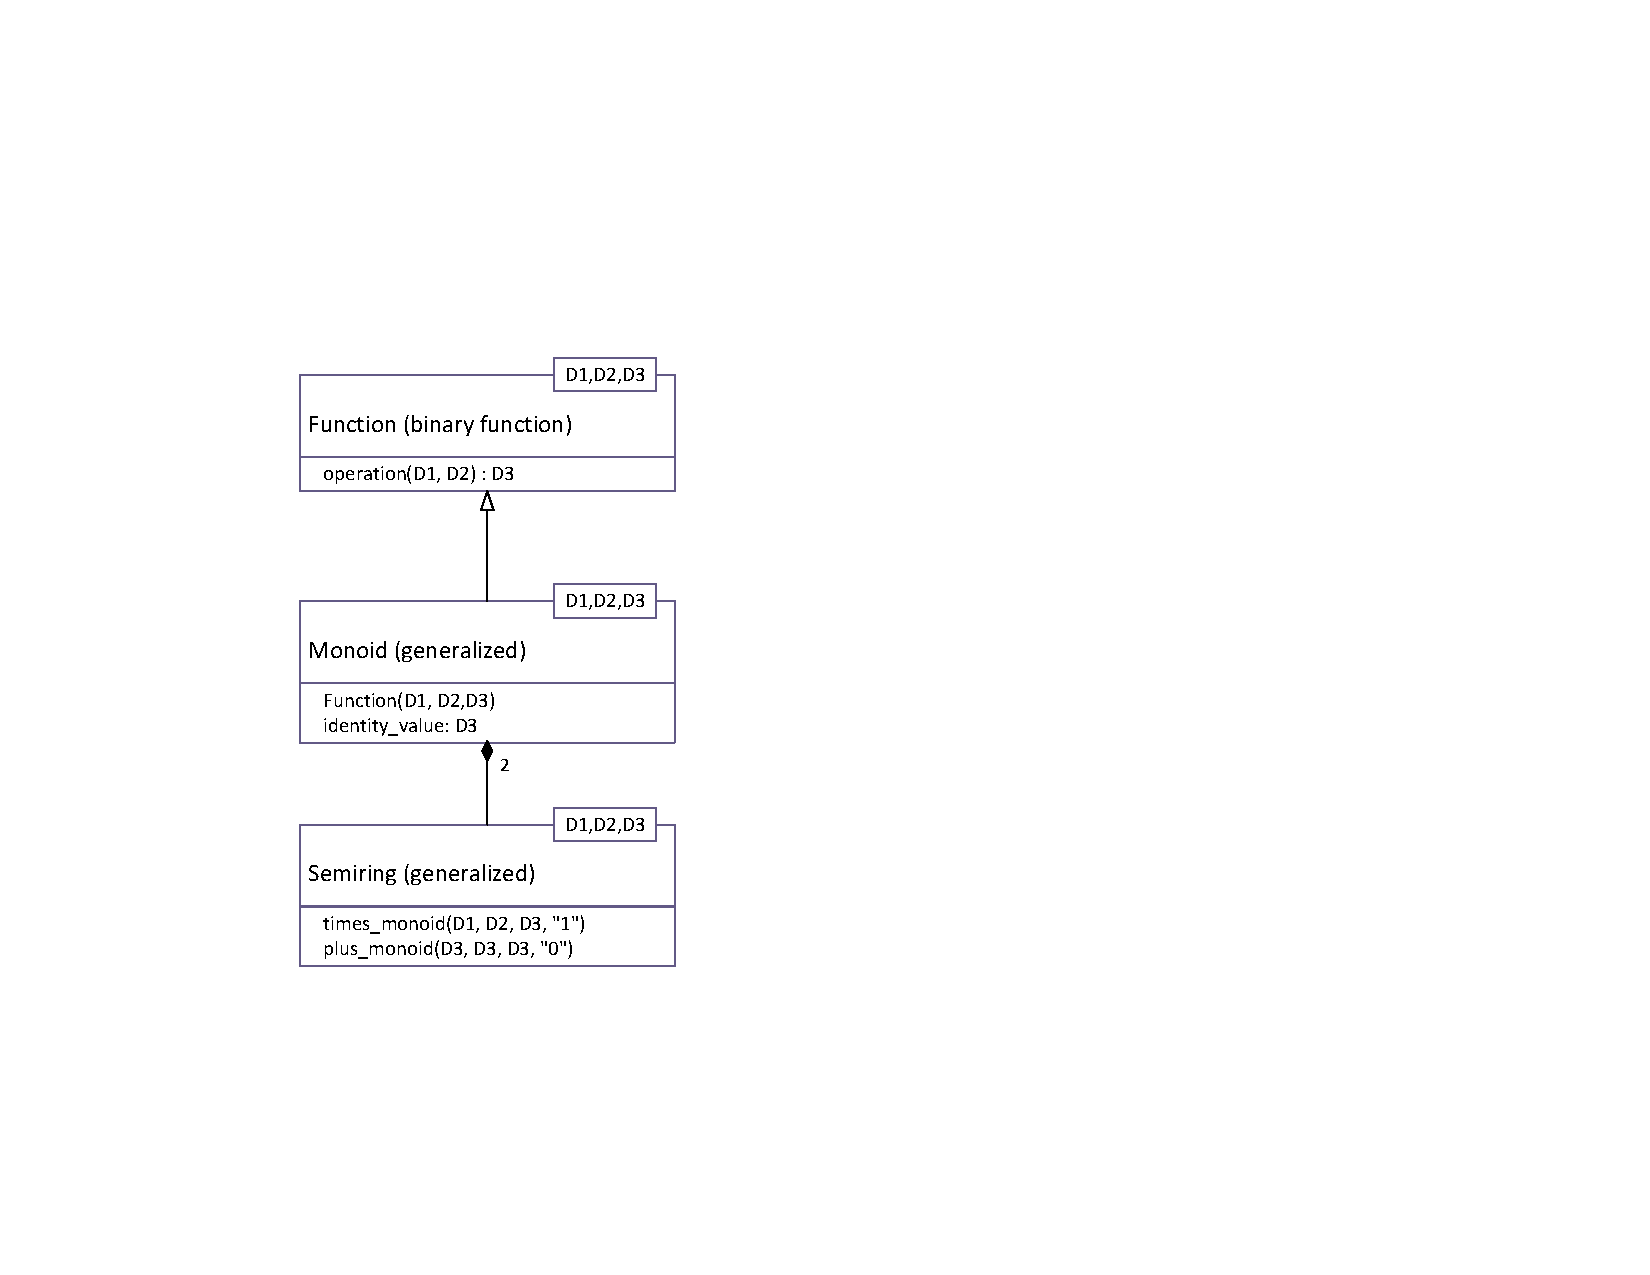
\includegraphics[width=1.0\linewidth,trim=0in 2in 0in 2in]{Algebra_Hierarchy.pdf}
\end{center}
\caption{Hierarchy of object classes in GraphBLAS algebra.}
\label{Fig:AlgebraHierarchy}
\hrule
\end{figure}

\subsection{Vectors}

\scott{Is this strictly sparse vector?} \jose{It is a GraphBLAS vector.}

A vector $\vector{v} = \langle D, N, \{ (i,v_i) \} \rangle$ is defined
by a domain $D$, a size $N>0$ and a set of tuples $(i,v_i)$ where
$0 \leq i < N$ and $v_i \in D$. A particular value of $i$ can only
appear at most once in $\vector{v}$. We define $\bold{n}(\vector{v}) =
N$ and $\bold{L}(\vector{v}) = \{ (i,v_i) \}$. We also define the set
$\vector{i(\vector{v})} = \{ i : (i,v_i) \in \bold{L}(\vector{v}) \}$,
and $\bold{D}(\vector{v}) = D$.

\comment{
\ajy{Overloaded use of $\vector{v}$ in the definition.} \jose{Fixed
through explicitly different fonts.} \scott{OK TO REMOVE}

\ajy{Why not define in terms of $D^{N}$} \jose{It is possible, but seems
more complicated to me.} \scott{OK TO REMOVE}
}

\scott{[snip] If we have a strictly 1D structure,
I believe we must give it an implicit orientation for matrix operations
(I prefer column vector) and discuss all the other vector operations
proposed a while back.}
\jose{I agree that vectors and matrices are more \emph{storage} than
anything else. But I don't think we should add any more properties (\eg,
orientation) than strictly necessary.}

\subsection{Matrices}
\label{Sec:Matrices}

\scott{Is this strictly sparse matrix?}

A matrix $\matrix{A} = \langle D, M, N,  \{ (i,j,A_{ij}) \} \rangle$ is
defined by a domain $D$. its number of rows $M>0$, its number of columns
$N>0$ and a set of tuples $(i,j,A_{ij})$ where $0 \leq i < M$, $0 \leq
j < N$, and $A_{ij} \in D$. A particular pair of values $i,j$ can only
appear at most once in $\matrix{A}$. We define $\bold{n}(\matrix{A})
= N$,  $\bold{m}(\matrix{A}) = M$ and $\bold{L}(\matrix{A}) = \{
(i,j,A_{ij}) \}$.  We also define the sets $\vector{i(\matrix{A})} = \{
i : \exists (i,j,A_{ij}) \in \matrix{A} \}$ and $\vector{j(\matrix{A})}
= \{ j : \exists (i,j,A_{ij}) \in \matrix{A} \}$.  (These are the sets
of nonempty rows and columns of $\matrix{A}$, respectively.)  Finally,
$\bold{D}(\matrix{A}) = D$.

\comment{
\ajy{Overloaded use of $\matrix{A}$ in the definition.}
\jose{Fixed through different fonts.}  \scott{OK TO REMOVE}

\ajy{Why not define in terms of $D^{M \times N}$.}
\jose{It seems more complicated to me.}  \scott{OK TO REMOVE}
}

If $\matrix{A}$ is a matrix and $0 \leq j < N$, then $\matrix{A}(:,j)
= \langle D, M, \{(i,A_{ij}) : (i,j,A_{ij}) \in \bold{L}(\matrix{A})
\} \rangle$ is a vector called the $j$-th \emph{column}
of $\matrix{A}$. Correspondingly, if $\matrix{A}$ is a matrix and
$0 \leq i < M$, then $\matrix{A}(i,:) = \langle D, N, \{(j,A_{ij}) :
(i,j,A_{ij}) \in \bold{L}(\matrix{A}) \} \rangle$ is a vector called
the $i$-th \emph{row} of $\matrix{A}$.

\subsection{Descriptors}

\jose{This was supposed to be just a conceptual introduction to
\emph{Descriptors}. We definitely need more detail. We can add it here
or save for the Section~\ref{Sec:Methods}.}

Descriptors are used as input parameters in various GraphBLAS methods to
provide more details of the operation to be performed by those methods.
In particular, descriptors specify how the other input parameters
should be processed before the main operation of a method is performed.
For example, a descriptor may specify that a particular input matrix
needs to be transposed or that a mask needs to be inverted before using
it in the operation. Some methods may also allow additional processing
of the result before generating the final output parameter.

\scott{'inverted' above is ambiguous, we need to define a better term
like "structural complement".  Further we should specify behaviour if
the mask is a dense container not just when it is sparse.}

For the purpose of constructing descriptors, the parameters of a method
are identified by specific names. The output parameter (typically
the first parameter in a GraphBLAS method) is {\sf OUTP}.  The input
parameters are named {\sf ARG0}, {\sf ARG1}, {\sf ARG2} and so on from
the first input parameter to the last. The mask (typically the next to
last parameter in a method) is named {\sf MASK}. Finally, the descriptor
(typically the last parameter in a method) is not named, since GraphBLAS
does not support modifications of descriptors themselves.

\scott{Is negate/invert/structural complement only restricted to masks?}

\scott{We must specify the behaviour of the descriptor's transpose.
E.g. is it allowed to mutate the operand for the duration of the
operation, or is this strictly a flag that affects the operation only --
how it accesses the operand's values?}

%==============================================================================================
%==============================================================================================

\section{Methods}
\label{Sec:Methods}

%==============================================================================================
\subsection{Algebra Methods}


\subsubsection{Create new function ({\sf Function\_new})}

Creates a new function with specified domain, operations and elements.

\paragraph{C99 Syntax}

\begin{verbatim}
#include "GraphBLAS.h"
GrB_info GrB_Function_new(GrB_Function *s,GrB_type t1, GrB_type t2, GrB_type t3,
                        GrB_operation a)
\end{verbatim}

GrB\_operation is a typedef to a standard C \emph{function pointer}.


\subsubsection{Create new monoid ({\sf Monoid\_new})}

Creates a new monoid with specified domain, operations and elements.

\paragraph{C99 Syntax}

\begin{verbatim}
#include "GraphBLAS.h"
GrB_info GrB_Monoid_new(GrB_Monoid *s,GrB_type t1, GrB_type t2, GrB_type t3,
                        GrB_operation a, <type> z)
\end{verbatim}

\paragraph{Input Parameters}

\begin{itemize}
	\item[{\sf t1}] The type defining the first domain of the monoid being created. Should be one of the predefined
	GraphBLAS types in Table~\ref{Tab:PredefinedTypes}, or a user created type.
	\item[{\sf t2}] The type defining the second domain of the monoid being created. Should be one of the predefined
	GraphBLAS types in Table~\ref{Tab:PredefinedTypes}, or a user created type.
	\item[{\sf t3}] The type defining the third domain of the monoid being created. Should be one of the predefined
	GraphBLAS types in Table~\ref{Tab:PredefinedTypes}, or a user created type.
	\item[{\sf a}] The additive operation of the monoid.
	\item[{\sf z}] The $0$ element of the monoid. Must be of type corresponding to {\sf t3} as per Table~\ref{Tab:PredefinedTypes}.
\end{itemize}

\paragraph{Output Parameter}

\begin{itemize}
	\item[{\sf s}] Identifier of the newly created monoid.
\end{itemize}

\paragraph{Return Value}

\begin{tabular}{rl} 
{\sf GrB\_SUCCESS} 	& operation completed successfully \\
{\sf GrB\_PANIC}	& unknown internal error \\
{\sf GrB\_OUTOFMEM}	& not enough memory available for operation \\
\end{tabular}

\paragraph{Description}

Creates a new monoid $S = \langle \bold{D}({\sf t1}), \bold{D}({\sf t2}), \bold{D}({\sf t3}), {\sf a}, {\sf z} \rangle$ and
returns its identifier in {\sf s}.


\subsubsection{Create new semiring ({\sf Semiring\_new})}

Creates a new semiring with specified domain, operations and elements.

\paragraph{C99 Syntax}

\begin{verbatim}
#include "GraphBLAS.h"
GrB_info GrB_Semiring_new(GrB_Semiring *s,GrB_type t1, GrB_type t2, GrB_type t3,
                       GrB_operation a,GrB_operation m, <type> z[, <type> o]))
\end{verbatim}

\scott{This signature is a little confusing partially because we have not been explicit with the domain/type specifications earlier. 
If the GrB\_type is the name of an enum for domains (not types) then I would suggest calling it GrB\_domain.  Not sure how {\sf ti} 
can be used as both a type and a parameter and may be related to the domain/type issue.}

\paragraph{Input Parameters}

\begin{itemize}
	\item[{\sf t1}] The type defining the first domain of the semiring being created. Should be one of the predefined
	GraphBLAS types in Table~\ref{Tab:PredefinedTypes}, or a user created type.
	\item[{\sf t2}] The type defining the second domain of the semiring being created. Should be one of the predefined
	GraphBLAS types in Table~\ref{Tab:PredefinedTypes}, or a user created type.
	\item[{\sf t3}] The type defining the third domain of the semiring being created. Should be one of the predefined
	GraphBLAS types in Table~\ref{Tab:PredefinedTypes}, or a user created type.
	\item[{\sf a}] The additive operation of the semiring.
	\item[{\sf m}] The multiplicative operation of the semiring.
	\item[{\sf z}] The $0$ element of the semiring. Must be of type corresponding to {\sf t3} as per Table~\ref{Tab:PredefinedTypes}.
	\item[{\sf o}] The $1$ element of the semiring. Must be of type corresponding to {\sf t3} as per Table~\ref{Tab:PredefinedTypes}.
\end{itemize}

\paragraph{Output Parameter}

\begin{itemize}
	\item[{\sf s}] Identifier of the newly created semiring.
\end{itemize}

\paragraph{Return Value}

\begin{tabular}{rl} 
{\sf GrB\_SUCCESS} 	& operation completed successfully \\
{\sf GrB\_PANIC}	& unknown internal error \\
{\sf GrB\_OUTOFMEM}	& not enough memory available for operation \\
\end{tabular}

\paragraph{Description}

Creates a new semiring $S = \langle \bold{D}({\sf t1}), \bold{D}({\sf t2}), \bold{D}({\sf t3}), {\sf a}, {\sf m}, {\sf z}, {\sf o} \rangle$ and
returns its identifier in {\sf s}.



%==============================================================================================
\subsection{Vector Methods}

\subsubsection{Create new vector ({\sf Vector\_new})}

Creates a new vector with specified domain and size.

\paragraph{C99 Syntax}

\begin{verbatim}
#include "GraphBLAS.h"
GrB_info GrB_Vector_new(GrB_Vector *v,GrB_type t,GrB_index n)
\end{verbatim}

\paragraph{Input Parameters}

\begin{itemize}
	\item[{\sf t}] The type defining the domain of the vector being created. Should be one of the predefined
	GraphBLAS types in Table~\ref{Tab:PredefinedTypes}, or a user created type.
	\item[{\sf n}] The size of the vector being created.
\end{itemize}

\paragraph{Output Parameter}

\begin{itemize}
	\item[{\sf v}] Identifier of the newly created vector.
\end{itemize}

\paragraph{Return Value}

\begin{tabular}{rl} 
{\sf GrB\_SUCCESS} 	& operation completed successfully \\
{\sf GrB\_PANIC}	& unknown internal error \\
{\sf GrB\_OUTOFMEM}	& not enough memory available for operation \\
\end{tabular}

\paragraph{Description}

Creates a new vector $\vector{v}$ of domain $D({\sf t})$, size {\sf n}, and
empty $L(\vector{v})$. It return in {\sf v} this vector $\vector{v}$.



%==============================================================================================
\subsection{Matrix Methods}

\subsubsection{Number of rows in a matrix ({\sf Matrix\_nrows})}

Retrieve the number of rows in a matrix.

\paragraph{C99 Syntax}

\begin{verbatim}
#include "GraphBLAS.h"
GrB_info GrB_Matrix_nrows(GrB_index *m,GrB_Matrix A)
\end{verbatim}

\paragraph{Input Parameters}

\begin{itemize}
	\item[{\sf A}] Matrix being queried.
\end{itemize}

\paragraph{Output Parameters}
\begin{itemize}
	\item[{\sf m}] The number of rows in the matrix.
\end{itemize}

\paragraph{Return Value}

\begin{tabular}{rl}
{\sf GrB\_SUCCESS}	& operation completed successfully \\
{\sf GrB\_PANIC}	& unknown internal error \\
{\sf GrB\_NOMATRIX}	& matrix does not exist \\
\end{tabular}

\paragraph{Description}

Return in {\sf m} the number of rows (parameter $M$ in Section~\ref{Sec:Matrices}) in matrix {\sf A}.


\subsubsection{Number of columns in a matrix ({\sf Matrix\_ncols})}

Placeholder

\subsubsection{Number of stored elements in a sparse matrix ({\sf Matrix\_nnz})}

Placeholder

%==============================================================================================
\subsection{Descriptor Methods}

\subsubsection{Create new descriptor ({\sf Descriptor\_new})}

Creates a new (empty) descriptor.

\paragraph{C99 Syntax}

\begin{verbatim}
#include "GraphBLAS.h"
GrB_info GrB_Descriptor_new(GrB_Descriptor *d)
\end{verbatim}

\paragraph{Output Parameters}

\begin{itemize}
	\item[{\sf d}] Identifier of new descriptor created.
\end{itemize}

\paragraph{Return Value}

\begin{tabular}{rl} 
{\sf GrB\_SUCCESS} 	& operation completed successfully \\
{\sf GrB\_PANIC}	& unknown internal error \\
{\sf GrB\_OUTOFMEM}	& not enough memory available for operation \\
{\sf GrB\_MISMATCH}	& mismatch between field and new value
\end{tabular}

\paragraph{Description}

Returns in {\sf d} the identifier of a newly created empty descriptor.
A newly created descriptor can be populated with calls to {\sf
Descriptor\_set}.

\subsubsection{Set content of descriptor ({\sf Descriptor\_set})}

\comment{
\scott{Naming nit: I propose {\sf Descriptor\_set}.  "adding" implies
accumulation (OR) of flags across many calls.  Allowing only set which
overwrites any existing values is simpler.} \jose{Agreed and modified.}  \scott{OK TO REMOVE}
}

Sets the content (details of an operation) for a field of an existing
descriptor.

\paragraph{C99 Syntax}

\begin{verbatim}
#include "GraphBLAS.h"
GrB_info GrB_Descriptor_set(GrB_Descriptor d,GrB_Field f,GrB_Value v)
\end{verbatim}

\paragraph{Input Parameters}

\begin{itemize}
	\item[{\sf d}] The descriptor being modified by this method.
	\item[{\sf f}] The descriptor field being set.
	\item[{\sf v}] New value for the field being set.
\end{itemize}

\paragraph{Return Value}

\begin{tabular}{rl} 
{\sf GrB\_SUCCESS} 	& operation completed successfully \\
{\sf GrB\_PANIC}	& unknown internal error \\
{\sf GrB\_OUTOFMEM}	& not enough memory available for operation \\
{\sf GrB\_MISMATCH}	& mismatch between field and new value
\end{tabular}

\paragraph{Description}

The fields of a descriptor include: {\sf GrB\_OUTP} for the 
output parameter (result) of a method; {\sf GrB\_MASK} for the mask
argument to a method; {\sf GrB\_ARG0} through {\sf GrB\_ARG9} for
the input parameters (from first to last) of a method.

Valid values for a field of a descriptor are as follows:

\begin{tabular}{rl} 
{\sf GrB\_NOP} 	& no operation to be performed for the corresponding parameter \\
{\sf GrB\_LNOT}	& \parbox[t]{5in}{compute the logical inverse \scott{structural complement?} of the corresponding parameter}  \\
{\sf GrB\_TRAN}	& compute the transpose of the corresponding parameter (for matrices) \\
{\sf GrB\_ACC}  & accumulate result of operation to current values in destination (for output parameter) \\
{\sf GrB\_CAST} & \parbox[t]{5in}{allow casting of values from input parameters to input domains of operation
                  or from output domain of operation to output parameter. (Otherwise, mismatching domains will cause a run-time error.)}
\end{tabular}

\scott{GrB\_LNOT clashes with operator in Table 2}

\ajy{GrB\_LNOT: logical inverse of non-mask parameters can be implemented by modifying the operators; therefore consider restricting this to masks only.}
\jose{I am OK with restricting {\sf GrB\_LNOT} to masks only.}

It is possible to specify a combination of values for a field. For 
example, if a matrix is to be both transposed and logically inverted
(element by element), one would use the field value
${\sf GrB\_TRAN} \mid {\sf GrB\_LNOT}$. 



%==============================================================================================
\subsection{GraphBLAS Operations}

\subsubsection{Store elements from tuples into a matrix ({\sf buildMatrix})}

Placeholder

\subsubsection{Extract tuples from a matrix ({\sf extractTuples})}

Placeholder

\subsubsection{Transpose rows and columns of a matrix ({\sf transpose})}

Placeholder

\subsubsection{Matrix-matrix multiply ({\sf mXm})}

Placeholder

\subsubsection{Vector-matrix multiply ({\sf vXm})}

Multiplies a vector by a matrix within an semiring. The result is a vector.

\paragraph{C99 Syntax}

\begin{verbatim}
#include "GraphBLAS.h"
GrB_info GrB_vxm(GrB_Vector *u, const GrB_Semiring s, const GrB_Vector v, 
                 const GrB_Matrix A[, const GrB_Vector m[, const GrB_Descriptor d]])
\end{verbatim}

\ajy{Should {\sf u} parameter have {\tt restrict} keyword?}
\jose{I don't see the value here. The implementors are free
to specialize the implementation when the matrices and
vectors do not overlap.}

\paragraph{Input Parameters}

\begin{itemize}
	\item[{\sf s}] ({\sf ARG0}) Semiring used in the vector-matrix
	multiply.

	\item[{\sf v}] ({\sf ARG1}) Vector to be multiplied.

	\item[{\sf A}] ({\sf ARG2}) Matrix to be multiplied.

	\item[{\sf m}] ({\sf MASK}) Operation mask (optional). The mask
	specifies which elements of the result vector are to be computed.
	If no mask is necessary (i.e., compute all elements of result
	vector), {\sf GrB\_NULL} can be used or the mask can be omitted.

	\item[{\sf d}] Operation descriptor (optional). The descriptor
	is used to specify details of the operation, such as transpose
	the matrix or not, invert the mask or not (see below). If a
	\emph{default} descriptor is desired, {\sf GrB\_NULL} can be
	used or the descriptor can be omitted.
\end{itemize}

\ajy{Can {\sf v} and {\sf m} refer to the same container?}
\ajy{Should ({\sf u} and {\sf v}) or ({\sf u} and {\sf m} NOT refer to the same container...use restrict?}
\jose{Don't see the value of restricting use at this level. All thse containers
are opaque, which means the implementation has full control. The {\bf Description} below
give a very specific semantics irrespective of overlap.}

\paragraph{Output Parameter}

\begin{itemize}
	\item[{\sf u}] ({\sf OUTP}) Address of result vector.
\end{itemize}

\paragraph{Return Value}

\scott{We should specify anything that we can about the behaviour/program state when any error condition is returned.  What gaurantees are we giving (think consistency models)?  Definitely related to mutability question earlier.}

\begin{tabular}{rl} 
{\sf GrB\_SUCCESS} 	& operation completed successfully \\
{\sf GrB\_PANIC}	& unknown internal error \\
{\sf GrB\_OUTOFMEM}	& not enough memory available for operation \\
{\sf GrB\_MISMATCH}	& mismatch among vectors, matrix and/or semiring
\end{tabular}

\scott{More return values possible: domain/type mismatches, dimension mismatches}
\jose{How much detail do we want?}
\scott{{\sf DOMAIN\_MISMATCH, DIMENSION\_MISMATCH} at least.}

\paragraph{Description}

Vectors $\vector{v}, \vector{m}$ and matrix $\matrix{A}$ are computed from
input parameters {\sf v}, {\sf m} and {\sf A}, respectively, as specified
by descriptor {\sf d}. (See below for the properties of a descriptor. In
the simplest form, these are just copies, but additional preprocessing,
including casting, can be specified.)  $\bold{D}(\vector{v}) =
\bold{D}_1({\sf s})$ and $\bold{D}(\matrix{A}) = \bold{D}_2({\sf s})$.
$\bold{D}(\vector{m}) = {\sf GrB\_BOOL}$.  If {\sf m} is {\sf GrB\_NULL}
then $\vector{m}$ is a Boolean vector of size $\bold{n}(\vector{A})$
and with all elements set to {\sf true}.

If either $\vector{v}, \vector{m}$ or $\matrix{A}$ cannot be computed
from the input parameters as described above, the method returns {\sf
GrB\_MISMATCH}.

A consistency check is performed to verify that $\bold{n}(\vector{v})
= \bold{m}(\matrix{A})$ and $\bold{n}(\vector{m}) =
\bold{n}(\matrix{A})$. If a consistency check fails, the operation is
aborted and the method returns {\sf GrB\_MISMATCH}.

A new vector $\vector{u} = \langle \bold{D}_3({\sf s}),
\bold{n}(\matrix{A}), \bold{L}(\vector{u}) = \{(i,u_i) : \vector{m}(i)
= {\sf true} \} \rangle$ is created.  The value of each of its elements
is computed by $u_i = \bigoplus_{j \in \vector{i}(\vector{v}) \cap
\vector{i}(\matrix{A}(:,i))} (\vector{v}(j) \otimes \matrix{A}(j,i))$,
where $\oplus$ and $\otimes$ are the additive and multiplicative
operations of semiring {\sf s}, respectively.  If $\vector{i}(\vector{v})
\cap \vector{i}(\matrix{A}(:,i)) = \emptyset$ then the pair $(i,u_i)$
is not included in $\bold{L}(\vector{u})$.

Finally, output parameter {\sf u} is computed from vector $\vector{u}$
as specified by descriptor {\sf d}. (Again, in the simplest case this
is just a copy, but additional postprocessing, including casting and
accumulation of result values, can be specified.)  A consistency check is
performed to verify that $\bold{n}({\sf u}) = \bold{n}(\vector{u})$. If
the consistency check fails, the operation is aborted and the method
return {\sf GrB\_MISMATCH}.

\scott{We need a more explicit discussion/specification regarding
masks and accumulation and their interaction (perhaps the diagram Manoj
projected at the SC15 BoF.} \jose{Agree. Need to find the proper place
for it.}

\scott{Is accumulation restricted to the use of the $\oplus$ operation
of the {\sf s} argument?  If so, add to the specification.} \jose{Yes,
accumulation is restricted to $\oplus$. Again, need to find the right
place for the specification.}

\subsubsection{Matrix-vector multiply ({\sf mXv})}

Multiplies a matrix by a vector within a semiring. The result is a vector.

\paragraph{C99 Syntax}

\begin{verbatim}
#include "GraphBLAS.h"
GrB_info GrB_mxv(GrB_Vector *u, const GrB_Semiring s, const GrB_Matrix A, 
                 const GrB_vector v[, const GrB_Vector m[, const GrB_Descriptor d]])
\end{verbatim}

\paragraph{Input Parameters}

\begin{itemize}
	\item[{\sf s}] ({\sf ARG0}) Semiring used in the vector-matrix
	multiply.

	\item[{\sf A}] ({\sf ARG1}) Matrix to be multiplied.

	\item[{\sf v}] ({\sf ARG2}) Vector to be multiplied.

	\item[{\sf m}] ({\sf MASK}) Operation mask (optional). The mask
	specifies which elements of the result vector are to be computed.
	If no mask is necessary (i.e., compute all elements of result
	vector), {\sf GrB\_NULL} can be used or the mask can be omitted.

	\item[{\sf d}] Operation descriptor (optional). The descriptor
	is used to specify details of the operation, such as transpose
	the matrix or not, invert the mask or not (see below). If a
	\emph{default} descriptor is desired, {\sf GrB\_NULL} can be
	used or the descriptor can be omitted.
\end{itemize}

\paragraph{Output Parameter}

\begin{itemize}
	\item[{\sf u}] ({\sf OUTP}) Address of result vector.
\end{itemize}

\paragraph{Return Value}

\begin{tabular}{rl} 
{\sf GrB\_SUCCESS} 	& operation completed successfully \\
{\sf GrB\_PANIC}	& unknown internal error \\
{\sf GrB\_OUTOFMEM}	& not enough memory available for operation \\
{\sf GrB\_MISMATCH}	& mismatch among vectors, matrix and/or semiring
\end{tabular}

\paragraph{Description}

Vectors $\vector{v}, \vector{m}$ and matrix $\matrix{A}$ are computed from
input parameters {\sf v}, {\sf m} and {\sf A}, respectively, as specified
by descriptor {\sf d}. (See below for the properties of a descriptor. In
the simplest form, these are just copies, but additional preprocessing,
including casting, can be specified.)  $\bold{D}(\vector{v}) =
\bold{D}_1({\sf s})$ and $\bold{D}(\matrix{A}) = \bold{D}_2({\sf s})$.
$\bold{D}(\vector{m}) = {\sf GrB\_BOOL}$.  If {\sf m} is {\sf GrB\_NULL} or omitted,
then $\vector{m}$ is a Boolean vector of size $\bold{n}(\vector{A})$
and with all elements set to {\sf true}.

If either $\vector{v}, \vector{m}$ or $\matrix{A}$ cannot be computed
from the input parameters as described above, the method returns {\sf
GrB\_MISMATCH}.

A consistency check is performed to verify that $\bold{n}(\vector{v})
= \bold{n}(\matrix{A})$ and $\bold{n}(\vector{m}) =
\bold{m}(\matrix{A})$. If a consistency check fails, the operation is
aborted and the method returns {\sf GrB\_MISMATCH}.

A new vector $\vector{u} = \langle \bold{D}_3({\sf s}),
\bold{m}(\matrix{A}), \bold{L}(\vector{u}) = \{(i,u_i) : \vector{m}(i)
= {\sf true} \} \rangle$ is created.  The value of each of its elements
is computed by $u_i = \bigoplus_{j \in \vector{i}(\vector{v}) \cap
\vector{i}(\matrix{A}(i,:))} (\matrix{A}(i,j)) \otimes \vector{v}(j)$,
where $\oplus$ and $\otimes$ are the additive and multiplicative
operations of semiring {\sf s}, respectively.  If $\vector{i}(\vector{v})
\cap \vector{i}(\matrix{A}(:,i)) = \emptyset$ then the pair $(i,u_i)$
is not included in $\bold{L}(\vector{u})$.

Finally, output parameter {\sf u} is computed from vector $\vector{u}$
as specified by descriptor {\sf d}. (Again, in the simplest case this
is just a copy, but additional postprocessing, including casting and
accumulation of result values, can be specified.)  A consistency check is
performed to verify that $\bold{n}({\sf u}) = \bold{n}(\vector{u})$. If
the consistency check fails, the operation is aborted and the method
return {\sf GrB\_MISMATCH}.


\subsubsection{Element-wise multiplication ({\sf eWiseMult})}

{\bf Note:} The difference between {\sf ewiseadd} and {\sf ewisemult} is not about the semiring operation but how the index sets are treated.
 {\sf ewiseadd} returns an object whose indices are the ``union'' of the indices of the inputs whereas  
 {\sf ewisemult} returns an object whose indices are the ``intersection'' of the indices of the inputs. In both cases, the passed monoid (or function) operates on the 
 set of values from the intersection set. 
 
\paragraph{Vector variant}

Perform element-wise (general) multiplication on the elements of two vectors,
producing a third vector as result.

\subparagraph{C99 Syntax}

\begin{verbatim}
#include "GraphBLAS.h"
GrB_info GrB_ewisemult(GrB_Vector* w, const GrB_Semiring s, const GrB_Vector u,
         const GrB_Vector v[, const GrB_Vector m[, const GrB_Descriptor d]])
GrB_info GrB_ewisemult(GrB_Vector* w, const GrB_Monoid s, const GrB_Vector u,
         const GrB_Vector v[, const GrB_Vector m[, const GrB_Descriptor d]])
GrB_info GrB_ewisemult(GrB_Vector* w, const GrB_Function s, const GrB_Vector u,
         const GrB_Vector v[, const GrB_Vector m[, const GrB_Descriptor d]])
\end{verbatim}

\subparagraph{Input Parameters}

\begin{itemize}
	\item[{\sf s}] ({\sf ARG0}) Semiring/monoid/function used in the element-wise multiplication.

	\item[{\sf u}] ({\sf ARG1}) Left vector to be multiplied.

	\item[{\sf v}] ({\sf ARG2}) Right vector to be multiplied.

	\item[{\sf m}] ({\sf MASK}) Operation mask (optional). The mask
	specifies which elements of the result vector are to be computed.
	If no mask is necessary (i.e., compute all elements of result
	vector), {\sf GrB\_NULL} can be used or the mask can be omitted.

	\item[{\sf d}] Operation descriptor (optional). The descriptor
	is used to specify details of the operation, such as 
	invert the mask or not (see below). If a
	\emph{default} descriptor is desired, {\sf GrB\_NULL} can be
	used or the descriptor can be omitted.
\end{itemize}

\subparagraph{Output Parameter}

\begin{itemize}
	\item[{\sf w}] ({\sf OUTP}) Address of result vector.
\end{itemize}

\subparagraph{Return Value}

\begin{tabular}{rl} 
{\sf GrB\_SUCCESS} 	& operation completed successfully \\
{\sf GrB\_PANIC}	& unknown internal error \\
{\sf GrB\_OUTOFMEM}	& not enough memory available for operation \\
{\sf GrB\_MISMATCH}	& mismatch among vectors and/or semiring/monoid/function
\end{tabular}

\subparagraph{Description}

If {\sf s} is a semiring, then $\otimes = \bigotimes({\sf s})$. 
If {\sf s} is a monoid or function, then $\otimes = \bigoplus({\sf s})$.

Vectors $\vector{v}, \vector{m}$ and $\vector{u}$ are computed from
input parameters {\sf v}, {\sf m} and {\sf u}, respectively, as specified
by descriptor {\sf d}. (See below for the properties of a descriptor. In
the simplest form, these are just copies, but additional preprocessing,
including casting, can be specified.)  $\bold{D}(\vector{u}) =
\bold{D}_1({\sf s})$ and $\bold{D}(\vector{v}) = \bold{D}_2({\sf s})$.
$\bold{D}(\vector{m}) = {\sf GrB\_BOOL}$.  If {\sf m} is {\sf GrB\_NULL} or omitted,
then $\vector{m}$ is a Boolean vector of size $\bold{n}(\vector{u})$
and with all elements set to {\sf true}.

If either $\vector{v}, \vector{m}$ or $\vector{u}$ cannot be computed
from the input parameters as described above, the method returns {\sf
GrB\_MISMATCH}.

A consistency check is performed to verify that $\bold{n}(\vector{v})
= \bold{n}(\vector{u}) = \bold{n}(\vector{m})$. If a consistency
check fails, the operation is aborted and the method returns {\sf
GrB\_MISMATCH}.

A new vector $\vector{w} = \langle \bold{D}_3({\sf s}),
\bold{n}(\vector{u}), \bold{L}(\vector{w}) = \{(i,w_i)  \forall i \in
\vector{i}(\vector{v}) \cap \vector{i}(\vector{u}) : \vector{m}(i)
= {\sf true} \} \rangle$ is created.  The value of each of its
elements is computed by $w_i = \vector{u}(i) \otimes \vector{v}(i)$,
where $\otimes$ is as defined above for {\sf s}.
If $\vector{i}(\vector{v}) \cap \vector{i}(\vector{u}) = \emptyset$
then $\bold{L}(\vector{w}) = \emptyset$.

Finally, output parameter {\sf w} is computed from vector $\vector{w}$
as specified by descriptor {\sf d}. (Again, in the simplest case this
is just a copy, but additional postprocessing, including casting and
accumulation of result values, can be specified.)  A consistency check is
performed to verify that $\bold{n}({\sf w}) = \bold{n}(\vector{w})$. If
the consistency check fails, the operation is aborted and the method
return {\sf GrB\_MISMATCH}.

\subsubsection{Element-wise addition ({\sf eWiseAdd})}

{\bf Note:} The difference between {\sf ewiseadd} and {\sf ewisemult} is not about the semiring operation but how the index sets are treated.
 {\sf ewiseadd} returns an object whose indices are the ``union'' of the indices of the inputs whereas  
 {\sf ewisemult} returns an object whose indices are the ``intersection'' of the indices of the inputs. In both cases, the passed monoid (or function) operates on the 
 set of values from the intersection set. 

\paragraph{Vector variant}

Perform element-wise (general) addition on the elements of two vectors,
producing a third vector as result.

\subparagraph{C99 Syntax}

\begin{verbatim}
#include "GraphBLAS.h"
GrB_info GrB_ewiseadd(GrB_Vector* w, const GrB_Semiring s, const GrB_Vector u,
         const GrB_Vector v[, const GrB_Vector m[, const GrB_Descriptor d]])
GrB_info GrB_ewiseadd(GrB_Vector* w, const GrB_Monoid s, const GrB_Vector u,
         const GrB_Vector v[, const GrB_Vector m[, const GrB_Descriptor d]])
GrB_info GrB_ewiseadd(GrB_Vector* w, const GrB_Function s, const GrB_Vector u,
         const GrB_Vector v[, const GrB_Vector m[, const GrB_Descriptor d]])
\end{verbatim}

\subparagraph{Input Parameters}

\begin{itemize}
	\item[{\sf s}] ({\sf ARG0}) Semiring/monoid/function used in the element-wise addition.

	\item[{\sf u}] ({\sf ARG1}) Left vector to be added.

	\item[{\sf v}] ({\sf ARG2}) Right vector to be added.

	\item[{\sf m}] ({\sf MASK}) Operation mask (optional). The mask
	specifies which elements of the result vector are to be computed.
	If no mask is necessary (i.e., compute all elements of result
	vector), {\sf GrB\_NULL} can be used or the mask can be omitted.

	\item[{\sf d}] Operation descriptor (optional). The descriptor
	is used to specify details of the operation, such as 
	invert the mask or not (see below). If a
	\emph{default} descriptor is desired, {\sf GrB\_NULL} can be
	used or the descriptor can be omitted.
\end{itemize}

\subparagraph{Output Parameter}

\begin{itemize}
	\item[{\sf w}] ({\sf OUTP}) Address of result vector.
\end{itemize}

\subparagraph{Return Value}

\begin{tabular}{rl} 
{\sf GrB\_SUCCESS} 	& operation completed successfully \\
{\sf GrB\_PANIC}	& unknown internal error \\
{\sf GrB\_OUTOFMEM}	& not enough memory available for operation \\
{\sf GrB\_MISMATCH}	& mismatch among vectors, matrix and/or semiring/monoid/function
\end{tabular}

\subparagraph{Description}

If {\sf s} is a semiring, then $\oplus = \bigoplus({\sf s})$. 
If {\sf s} is a monoid or function, then $\oplus = \bigoplus({\sf s})$.

Vectors $\vector{v}, \vector{m}$ and $\vector{u}$ are computed from
input parameters {\sf v}, {\sf m} and {\sf u}, respectively, as specified
by descriptor {\sf d}. (See below for the properties of a descriptor. In
the simplest form, these are just copies, but additional preprocessing,
including casting, can be specified.)  $\bold{D}(\vector{u}) =
\bold{D}_3({\sf s})$ and $\bold{D}(\vector{v}) = \bold{D}_3({\sf s})$.
$\bold{D}(\vector{m}) = {\sf GrB\_BOOL}$.  If {\sf m} is {\sf GrB\_NULL} or omitted,
then $\vector{m}$ is a Boolean vector of size $\bold{n}(\vector{u})$
and with all elements set to {\sf true}.

If either $\vector{v}, \vector{m}$ or $\vector{u}$ cannot be computed
from the input parameters as described above, the method returns {\sf
GrB\_MISMATCH}.

A consistency check is performed to verify that $\bold{n}(\vector{v})
= \bold{n}(\vector{u}) = \bold{n}(\vector{m})$. If a consistency check fails, the operation is
aborted and the method returns {\sf GrB\_MISMATCH}.

A new vector $\vector{w} = \langle \bold{D}_3({\sf s}),
\bold{n}(\vector{u}), \bold{L}(\vector{w}) = \{(i,w_i)  \forall i \in
\vector{i}(\vector{v}) \cup \vector{i}(\vector{u}) : \vector{m}(i)
= {\sf true} \} \rangle$ is created.  The value of each of its
elements is computed by 
\[
w_i = \vector{u}(i) \oplus \vector{v}(i), \ \mbox{if}\  i \in  \vector{i}(\vector{v}) \cap \vector{i}(\vector{u})
\]
\[
w_i = \vector{u}(i) \ \mbox{if}\  i \in  \vector{i}(\vector{u}) - (\vector{i}(\vector{v}) \cap \vector{i}(\vector{u}))
\]
\[
w_i = \vector{v}(i) \ \mbox{if}\  i \in  \vector{i}(\vector{v}) - (\vector{i}(\vector{v}) \cap \vector{i}(\vector{u}))
\]
where $\oplus$ is as defined above for {\sf s}.
If $\vector{i}(\vector{v}) \cup \vector{i}(\vector{u}) = \emptyset$
then $\bold{L}(\vector{w}) = \emptyset$.

Finally, output parameter {\sf w} is computed from vector $\vector{w}$
as specified by descriptor {\sf d}. (Again, in the simplest case this
is just a copy, but additional postprocessing, including casting and
accumulation of result values, can be specified.)  A consistency check is
performed to verify that $\bold{n}({\sf w}) = \bold{n}(\vector{w})$. If
the consistency check fails, the operation is aborted and the method
return {\sf GrB\_MISMATCH}.

\subsubsection{Extract a sub-matrix from a larger matrix ({\sf extract})}

Placeholder

\subsubsection{Assign a matrix to a set of indices (sub-matrix) of a larger matrix ({\sf assign})}

\scott{these variants need to be discussed perhaps in the large group; not currently part of any prior document.}

\paragraph{Flat variant}

Set all the elements of a vector to a given value.

\begin{verbatim}
#include "GraphBLAS.h"
GrB_info GrB_assign(GrB_Vector *v,scalar s[,GrB_Vector m])
\end{verbatim}

\subparagraph{Input Parameters}

\begin{itemize}
	\item[{\sf v}] Vector to be assigned.
	\item[{\sf s}] Scalar value for the elements.
	\item[{\sf m}] (Optional) mask for assignment. \aydin{Maybe say in the document that GrB\_Vector's domain could only be GrB\_Index for this function} \jose{Any domain that can be cast to {\sf GrB\_BOOL} will do.}
\end{itemize}

\subparagraph{Return Value}

\begin{tabular}{rl}
{\sf GrB\_SUCCESS}	& operation completed successfully \\
{\sf GrB\_PANIC}	& unknown internal error \\
{\sf GrB\_NOVECTOR}	& vector does not exist \\
{\sf GrB\_MISMATCH}	& mismatch between vector domain and scalar type \\
\end{tabular}

\paragraph{Indexed variant}

Set some of the elements of a vector to a given value.
\scott{Set one element of...}

\subparagraph{C99 Syntax}

\begin{verbatim}
#include "GraphBLAS.h"
GrB_info GrB_assign(GrB_Vector *v,scalar s,GrB_index i)
\end{verbatim}

\subparagraph{Input Parameters}

\begin{itemize}
	\item[{\sf v}] Vector to be assigned.
	\item[{\sf s}] Scalar value for the elements.
	\item[{\sf i}] Index of element to be assigned
\end{itemize}

\subparagraph{Return Value}

\begin{tabular}{rl}
{\sf GrB\_SUCCESS}	& operation completed successfully \\
{\sf GrB\_PANIC}	& unknown internal error \\
{\sf GrB\_NOVECTOR}	& vector does not exist \\
{\sf GrB\_MISMATCH}	& mismatch between vector domain and scalar type \\
\end{tabular}

\subsubsection{Apply a unary function to the elements of a matrix ({\sf apply})}

Placeholder

\subsubsection{Perform a reduction across the elements of an object ({\sf reduce})}

Computes the reduction of the values of the elements of a vector or matrix.

\paragraph{Vector variant}

\subparagraph{C99 Syntax}

\begin{verbatim}
#include "GraphBLAS.h"
GrB_info GrB_reduce(scalar *t, const GrB_Semiring s, const GrB_Vector v
                    [, const GrB_Descriptor d])
GrB_info GrB_reduce(scalar *t, const GrB_Monoid s, const GrB_Vector v
                    [, const GrB_Descriptor d])
\end{verbatim}

\comment{
\scott{Should we use the space/semiring in place of the {\sf f} parameter
and just use the $\oplus$ or if an semiring consists of monoids this is
another place where a Monoid is appropriate.  Note that we must know the
identity value for the operation in order to store the correct value in
the scalar if the vector that you are reducing has not stored values.}
\jose{Yes, we should. Changed.}\scott{OK TO REMOVE}
}

\scott{Now we shift to the conversation about whether s is replaced with a
"relaxed monoid" or "binary function + identity"}

\subparagraph{Input Parameters}

\begin{itemize}
	\item[{\sf v}] Vector to be reduced.
	\item[{\sf s}] Semiring/monoid defining the reduction.
	\item[{\sf d}] Operation descriptor (optional).
\end{itemize}

\subparagraph{Output Parameters}

\begin{itemize}
	\item[{\sf t}] Value of the reduction. It must
	be a pointer to one of the types in 
	the left column of Table~\ref{Tab:PredefinedTypes} or
	{\tt void*}.
\end{itemize}

\subparagraph{Return Value}

\begin{tabular}{rl}
{\sf GrB\_SUCCESS}	& operation completed successfully \\
{\sf GrB\_PANIC}	& unknown internal error \\
{\sf GrB\_NOVECTOR}	& vector does not exist \\
{\sf GrB\_MISMATCH}	& mismatch between vector domain, scalar type or semiring/monoid \\
\end{tabular}

\subparagraph{Description}

Let $0 = \bold{0}({\sf s})$, whether ${\sf s}$ is a semiring or monoid.
Let $\oplus = \bigoplus({\sf s})$.

We must have $\bold{D}_3({\sf s}) = \bold{D}_1({\sf s})$.
Otherwise, the method returns {\sf GrB\_MISMATCH}.

Vector $\vector{v}$ is computed from input parameter ${\sf v}$ as
specified by descriptor {\sf d}. $\bold{D}(\vector{v}) = \bold{D}_2({\sf s})$
and $\bold{n}(\vector{v}) = \bold{n}({\sf v})$. If $\vector{v}$ cannot be computed
from the input parameters, the method returns {\sf GrB\_MISMATCH}.

A scalar variable $t$ such that $\bold{D}(t) = \bold{D_1}({\sf s})$ is
created and initialized $t \leftarrow \bold{0}({\sf s})$. 
We then compute the recurrence $t \leftarrow t \oplus v_i, \forall i \in \vector{i}(\vector{v})$.

Finally, output parameter {\sf t} is computed from scalar $t$.

%=============================================================================
\subsection{Utility Operations}

\subsubsection{Destroy object ({\sf free})}

Destroys a previously created GraphBLAS object.

\paragraph{C99 Syntax}

\begin{verbatim}
#include "GraphBLAS.h"
GrB_info GrB_free(GrB_Object o)
\end{verbatim}

\ajy{polymorphic?  is there where \_Generic is specified?}
\jose{This is \emph{one} of the polymorphic functions in the C API.
I changed the introduction to say that polymorphism must be supported by an
extensio of C99. {\tt \_Generic} is just one way of accomplishing that.}

\paragraph{Input Parameter}

\begin{itemize}
	\item[{\sf o}] GraphBLAS object to be destroyed. Can be a matrix, vector or descriptor.
\end{itemize}

\paragraph{Return Value}

\begin{tabular}{rl}
{\sf GrB\_SUCCESS}	& operation completed successfully \\
{\sf GrB\_PANIC}	& unknown internal error \\
{\sf GrB\_NOOBJECT}	& object does not exist \\
\end{tabular}


%=============================================================================
%=============================================================================

\appendix

\pagebreak
\nolinenumbers
\section{Example: breadth first search with GraphBLAS}
{\scriptsize
\lstinputlisting[language=C,numbers=left]{BFS5M.c}
}

\pagebreak
\nolinenumbers
\section{Example: betweenness centrality with GraphBLAS}
{\scriptsize
\lstinputlisting[language=C,numbers=left]{BC1M.c}
}

\comment{
\pagebreak
\linenumbers
\section{Algebraless option}

\subsection{Vector-matrix multiply ({\sf vxm})}

Multiplies a vector by a matrix. The result is a vector.

\paragraph{C99 Syntax}

\begin{verbatim}
#include "GraphBLAS.h"
GrB_info GrB_vxm(GrB_Vector *u, const GrB_operation f, const GrB_operation g,
         const GrB_Vector v, const GrB_Matrix A
         [, const GrB_Vector m[, const GrB_Descriptor d]])
\end{verbatim}

\paragraph{Input Parameters}

\begin{itemize}
	\item[{\sf f}] ({\sf ARG0}) Additive operation used in the vector-matrix
	multiply.

	\item[{\sf g}] ({\sf ARG1}) Multiplicative oepration useind in the vector-matrix multiply.

	\item[{\sf v}] ({\sf ARG2}) Vector to be multiplied.

	\item[{\sf A}] ({\sf ARG3}) Matrix to be multiplied.

	\item[{\sf m}] ({\sf MASK}) Operation mask (optional). The mask
	specifies which elements of the result vector are to be computed.
	If no mask is necessary (i.e., compute all elements of result
	vector), {\sf GrB\_NULL} can be used or the mask can be omitted.

	\item[{\sf d}] Operation descriptor (optional). The descriptor
	is used to specify details of the operation, such as transpose
	the matrix or not, invert the mask or not (see below). If a
	\emph{default} descriptor is desired, {\sf GrB\_NULL} can be
	used or the descriptor can be omitted.
\end{itemize}

\paragraph{Output Parameter}

\begin{itemize}
	\item[{\sf u}] ({\sf OUTP}) Address of result vector.
\end{itemize}

\paragraph{Return Value}

\begin{tabular}{rl} 
{\sf GrB\_SUCCESS} 	& operation completed successfully \\
{\sf GrB\_PANIC}	& unknown internal error \\
{\sf GrB\_OUTOFMEM}	& not enough memory available for operation \\
{\sf GrB\_MISMATCH}	& mismatch among vectors, matrix and/or algebra
\end{tabular}

\paragraph{Description}

Let $\otimes: D_1 \times D_2 \rightarrow D_3$ and $\oplus: D_3 \times
D_3 \rightarrow D_3$ be the operations defined by arguments {\sf f}
and {\sf g}, respectively.

Vectors $\vector{v}, \vector{m}$ and matrix $\matrix{A}$ are computed
from input parameters {\sf v}, {\sf m} and {\sf A}, respectively,
as specified by descriptor {\sf d}.  $\bold{D}(\vector{v}) = D_1$ and
$\bold{D}(\matrix{A}) = D_2$.  $\bold{D}(\vector{m}) = {\sf GrB\_BOOL}$.
If {\sf m} is {\sf GrB\_NULL} then $\vector{m}$ is a Boolean vector of
size $\bold{n}(\vector{A})$ and with all elements set to {\sf true}.

If either $\vector{v}, \vector{m}$ or $\matrix{A}$ cannot be computed
from the input parameters as described above, the method returns {\sf
GrB\_MISMATCH}.

A consistency check is performed to verify that $\bold{n}(\vector{v})
= \bold{m}(\matrix{A})$ and $\bold{n}(\vector{m}) =
\bold{n}(\matrix{A})$. If a consistency check fails, the operation is
aborted and the method returns {\sf GrB\_MISMATCH}.

A new vector $\vector{u} = \langle D_3, \bold{n}(\matrix{A}),
\bold{L}(\vector{u}) = \{(i,u_i) : \vector{m}(i) = {\sf true} \} \rangle$
is created.  The value of each of its elements is computed by $u_i =
\bigoplus_{j \in \vector{i}(\vector{v}) \cap \vector{i}(\matrix{A}(:,i))}
(\vector{v}(j) \otimes \matrix{A}(j,i))$.  If $\vector{i}(\vector{v})
\cap \vector{i}(\matrix{A}(:,i)) = \emptyset$ then the pair $(i,u_i)$
is not included in $\bold{L}(\vector{u})$.

Finally, output parameter {\sf u} is computed from vector $\vector{u}$
as specified by descriptor {\sf d}.  A consistency check is performed
to verify that $\bold{n}({\sf u}) = \bold{n}(\vector{u})$. If the
consistency check fails, the operation is aborted and the method return
{\sf GrB\_MISMATCH}.

\jose{The domains are now defined by the oeprations. Which means we need
different versions of common operations such as {\sf GrB\_PLUS}:
{\sf GrB\_PLUSI64} (for {\tt int64\_t}), {\sf GrB\_PLUSU64} (for {\tt uint64\_t}), {\sf GrB\_PLUSF64} (for {\tt double}),
{\sf GrB\_PLUSI32} (for {\tt int32\_t}), {\sf GrB\_PLUSU32} (for {\tt uint32\_t}), {\sf GrB\_PLUSF32} (for {\tt float}),
}

\pagebreak
\nolinenumbers
\section{Example: BFS with Algebraless-GraphBLAS}
{\scriptsize
\lstinputlisting[language=C,numbers=left]{BFS5AL.c}
}

\pagebreak
\nolinenumbers
\section{Example: BC with Algebraless-GraphBLAS}
{\scriptsize
\lstinputlisting[language=C,numbers=left]{BC1AL.c}
}

\pagebreak
\linenumbers
\section{Monoid option}

A GraphBLAS \emph{monoid} $M = \langle D_1,D_2,D_3,\oplus,0 \rangle$ is
defined by three domains $D_1$, $D_2$, $D_3$, an operation $\oplus:
D_1 \times D_2 \rightarrow D_3$, and an identity $0 \in D_1 \cap D_2$.
It is required that $D_1 \subseteq D_3$ and $D_2 \subseteq D_3$. For a given GraphBLAS monoid $M=\langle
D_1, D_2, D_3,\oplus,0 \rangle$ we define $\bold{D}_1(M) =
D_1$, $\bold{D}_2(M) = D_2$, $\bold{D}_3(M) = D_3$, $\bold{\bigoplus}(M)
= \oplus$ and $\bold{0}(S) = 0$.

\subsection{Element-wise multiplication ({\sf ewisemult})}

\subsubsection{Vector variant}

Perform element-wise (general) multiplication on the elements of two vectors,
producing a third vector as result.

\paragraph{C99 Syntax}

\begin{verbatim}
#include "GraphBLAS.h"
GrB_info GrB_ewisemult(GrB_Vector* w, const GrB_Monoid s, const GrB_Vector u,
         const GrB_Vector v[, const GrB_Vector m[, const GrB_Descriptor d]])
\end{verbatim}

\paragraph{Input Parameters}

\begin{itemize}
	\item[{\sf s}] ({\sf ARG0}) Monoid used in the vector-wise multiplication.

	\item[{\sf u}] ({\sf ARG1}) Left vector to be multiplied.

	\item[{\sf v}] ({\sf ARG2}) Right vector to be multiplied.

	\item[{\sf m}] ({\sf MASK}) Operation mask (optional). The mask
	specifies which elements of the result vector are to be computed.
	If no mask is necessary (i.e., compute all elements of result
	vector), {\sf GrB\_NULL} can be used or the mask can be omitted.

	\item[{\sf d}] Operation descriptor (optional). The descriptor
	is used to specify details of the operation, such as 
	invert the mask or not (see below). If a
	\emph{default} descriptor is desired, {\sf GrB\_NULL} can be
	used or the descriptor can be omitted.
\end{itemize}

\paragraph{Output Parameter}

\begin{itemize}
	\item[{\sf w}] ({\sf OUTP}) Address of result vector.
\end{itemize}

\paragraph{Return Value}

\begin{tabular}{rl} 
{\sf GrB\_SUCCESS} 	& operation completed successfully \\
{\sf GrB\_PANIC}	& unknown internal error \\
{\sf GrB\_OUTOFMEM}	& not enough memory available for operation \\
{\sf GrB\_MISMATCH}	& mismatch among vectors and/or algebra
\end{tabular}

\paragraph{Description}

Vectors $\vector{v}, \vector{m}$ and $\vector{u}$ are computed from
input parameters {\sf v}, {\sf m} and {\sf u}, respectively, as specified
by descriptor {\sf d}. (See below for the properties of a descriptor. In
the simplest form, these are just copies, but additional preprocessing,
including casting, can be specified.)  $\bold{D}(\vector{u}) =
\bold{D}_1({\sf s})$ and $\bold{D}(\vector{v}) = \bold{D}_2({\sf s})$.
$\bold{D}(\vector{m}) = {\sf GrB\_BOOL}$.  If {\sf m} is {\sf GrB\_NULL} or omitted,
then $\vector{m}$ is a Boolean vector of size $\bold{n}(\vector{u})$
and with all elements set to {\sf true}.

If either $\vector{v}, \vector{m}$ or $\vector{u}$ cannot be computed
from the input parameters as described above, the method returns {\sf
GrB\_MISMATCH}.

A consistency check is performed to verify that $\bold{n}(\vector{v})
= \bold{n}(\vector{u}) = \bold{n}(\vector{m})$. If a consistency
check fails, the operation is aborted and the method returns {\sf
GrB\_MISMATCH}.

A new vector $\vector{w} = \langle \bold{D}_3({\sf s}),
\bold{n}(\vector{u}), \bold{L}(\vector{w}) = \{(i,w_i)  \forall i \in
\vector{i}(\vector{v}) \cap \vector{i}(\vector{u}) : \vector{m}(i)
= {\sf true} \} \rangle$ is created.  The value of each of its
elements is computed by $w_i = \vector{u}(i) \otimes \vector{v}(i)$,
where $\otimes$ is the multiplicative operation of algebra {\sf s}.
If $\vector{i}(\vector{v}) \cap \vector{i}(\vector{u}) = \emptyset$
then $\bold{L}(\vector{w}) = \emptyset$.

Finally, output parameter {\sf w} is computed from vector $\vector{w}$
as specified by descriptor {\sf d}. (Again, in the simplest case this
is just a copy, but additional postprocessing, including casting and
accumulation of result values, can be specified.)  A consistency check is
performed to verify that $\bold{n}({\sf w}) = \bold{n}(\vector{w})$. If
the consistency check fails, the operation is aborted and the method
return {\sf GrB\_MISMATCH}.

\subsection{Perform a reduction across the elements of an object ({\sf reduce})}

Computes the reduction of the values of the elements of a vector or matrix.

\subsubsection{Vector variant}

\paragraph{C99 Syntax}

\begin{verbatim}
#include "GraphBLAS.h"
GrB_info GrB_reduce(scalar *t, const GrB_Monoid s, const GrB_Vector v)
\end{verbatim}

\paragraph{Input Parameters}

\begin{itemize}
	\item[{\sf v}] Vector to be reduced.
	\item[{\sf s}] Monoid defining the reduction.
\end{itemize}

\paragraph{Output Parameters}

\begin{itemize}
	\item[{\sf t}] Value of the reduction. It must
	be a pointer to one of the types in 
	the left column of Table~\ref{Tab:PredefinedTypes} or
	{\tt void*}.
\end{itemize}

\paragraph{Return Value}

\begin{tabular}{rl}
{\sf GrB\_SUCCESS}	& operation completed successfully \\
{\sf GrB\_PANIC}	& unknown internal error \\
{\sf GrB\_NOVECTOR}	& vector does not exist \\
{\sf GrB\_MISMATCH}	& mismatch between vector domain and scalar type \\
\end{tabular}

\pagebreak
\nolinenumbers
\section{Example: BC with Monoid option}
{\scriptsize
\lstinputlisting[language=C,numbers=left]{BC1M.c}
}
}

\pagebreak
\section{Objects}
%\Carl{Proposal: Associative definition to separate concepts of Function and Monoid. Wanted y'all to take a look before changing the section.}

The following objects (functions, monoids, and semirings) are presented in increasing generality.
The ``algebra generality rule'' of GraphBLAS states that a more general object can always be passed to
any function which requires a less general object. The restriction rules are explained in the respective sections of those objects.

\subsection{Functions}

A GraphBLAS \emph{function} $F = \langle D_1,D_2,D_3,\oplus \rangle$
is defined by three domains $D_1$, $D_2$, $D_3$, and an operation
$\oplus: D_1 \times D_2 \rightarrow D_3$.  For a given GraphBLAS function
$F=\langle D_1, D_2, D_3,\oplus \rangle$ we define $\bold{D}_1(F) = D_1$,
$\bold{D}_2(F) = D_2$, $\bold{D}_3(F) = D_3$, and $\bold{\bigoplus}(F)
= \oplus$.

\subsection{Monoids}

A GraphBLAS \emph{generalized monoid} (or \emph{monoid} for short) $M =
\langle D_1,\oplus,0 \rangle$ is defined by a single domain $D_1$, an 
\emph{associative} operation $\oplus: D_1 \times D_1 \rightarrow D_1$,
and an identity element $0 \in D_1$.  For a given GraphBLAS monoid $M=\langle
D_1,oplus,0 \rangle$ we define $\bold{D}_1(M) = D_1$, $\bold{\bigoplus}(M) =
\oplus$ and $\bold{0}(M) = 0$.  A GraphBLAS monoid is equivalent to 
the conventional \emph{monoid} algebraic structure.

Let $F = \langle D_1,D_1,D_1,\oplus \rangle$ be a GraphBLAS function
with element $0 \in D_1$.  Then $M = \langle F,0 \rangle = \langle
D_1,\oplus,0 \rangle$ is a GraphBLAS monoid.

Note: It is understood that \emph{associativity} is not guaranteed in IEEE 754 floating-point arithmetic. The authors relax associativity to a weaker form called \emph{reproducibility} defined as being able to attain reasonably accurate results (within an absolute error bound) regardless of the order of evaluation and ill-conditioning of the problem. Demmel and Nguyen have shown this to be achievable in IEEE 754 floating-point arithmetic~\cite{Demmel:2013:FRF}. \emph{Reproducibility} is an important property, because it provides a bound on absolute error when the order of evaluation is changed. Ability to change the order of evaluation is a must for parallel computation. Examples of key GraphBLAS operations that require associativity to run in parallel include {\mbox{\bf mXm}}, {\mbox{\bf mXv}} and {\mbox{\bf reduce}}.

\subsection{Semirings}

A GraphBLAS \emph{generalized semiring} (or \emph{semiring} for short)
$S=\langle D_1,D_2,D_3,\oplus,\otimes,0 [,1] \rangle$ is defined by
three domains $D_1$, $D_2$ and $D_3$, an additive operation $\oplus :
D_3 \times D_3 \rightarrow D_3$, 
a multiplicative operation $\otimes : D_1 \times D_2 \rightarrow
D_3$, an element $0 \in D_3$ and an optional element $1 \in D_3$.
For a given GraphBLAS semiring $S=\langle D_1,
D_2, D_3,\oplus,\otimes,0,1 \rangle$ we define $\bold{D}_1(S) = D_1$,
$\bold{D}_2(S) = D_2$, $\bold{D}_3(S) = D_3$, $\bold{\bigoplus}(S) =
\oplus$, $\bold{\bigotimes}(S) = \otimes$, $\zero(S) = 0$ and $\one(S) =
1$. We note that, in the special case of $D_1 = D_2 = D_3$, $1$ defined and the identity of $\otimes$,
and $0$ working as the $\oplus$ identity and $\otimes$ annihilator (\ie, $0 \otimes x = x
\otimes 0 = 0, \forall x \in D_3$), a GraphBLAS semiring reduces to the
conventional \emph{semiring} algebraic structure.

Let $M = \langle D_3, \otimes,1 \rangle$ and $A = \langle D_3,\oplus,0 \rangle$ be monoids.
Then $S= \langle A,M \rangle = \langle D_3,D_3,D_3,\oplus,\otimes,0,1 \rangle$
is a semiring.

Let $F = \langle D_1,D_2,D_3,\otimes \rangle$ be a function
and let $A = \langle D_3,\oplus,0 \rangle$ be a monoid,
then $S= \langle A,F \rangle = \langle D_1,D_2,D_3,\oplus,\otimes,0 \rangle$
is a semiring.

A UML diagram of the hierarchy of object classes in GraphBLAS
algebra (functions, monoids and semirings) is shown in 
Figure ~\ref{Fig:AlgebraHierarchyProposed}.

\begin{figure}[htb]
\hrule
\begin{center}
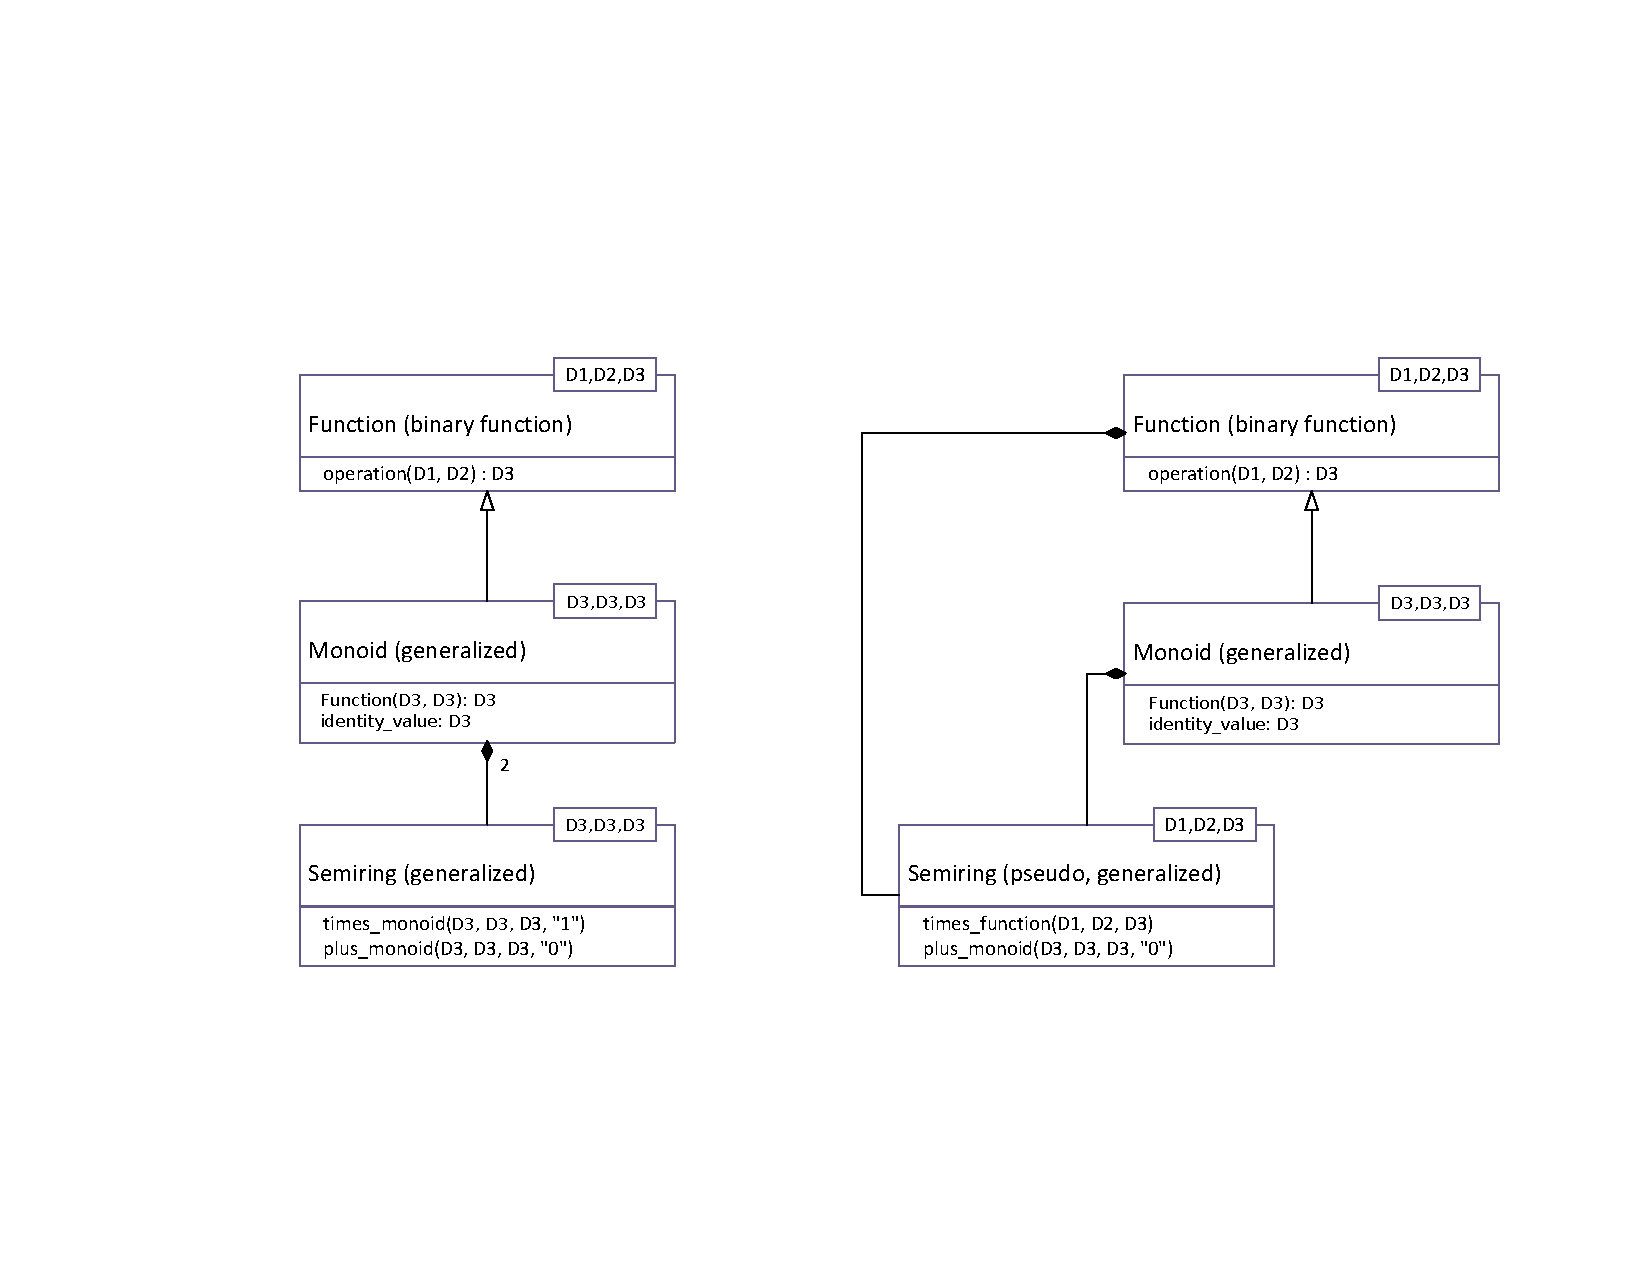
\includegraphics[width=1.0\linewidth,trim=0in 2in 0in 2in]{Algebra_Hierarchy_proposed.pdf}
\end{center}
\caption{Hierarchy of object classes in GraphBLAS algebra.}
\label{Fig:AlgebraHierarchyProposed}
\hrule
\end{figure}

\def\IEEEbibitemsep{3pt plus .5pt}
\bibliographystyle{IEEEtran}
\bibliography{refs}

\end{document}
